\documentclass[12pt,a4paper]{article}

% Packages
\usepackage[margin=2.5cm]{geometry}
\usepackage[utf8]{inputenc}
\usepackage[T1]{fontenc}
\usepackage{lmodern}
\usepackage{setspace}
\usepackage{amsmath,amssymb}
\usepackage{graphicx}
\graphicspath{{figures/}}
\usepackage{booktabs}
\usepackage{longtable}
\usepackage{float}
\usepackage{caption}
\usepackage{enumitem}
\usepackage{xcolor}
\usepackage{pdflscape}
\usepackage{tikz}
\usetikzlibrary{positioning}
\usepackage[colorlinks=true,linkcolor=blue!60!black,citecolor=blue!60!black,urlcolor=blue!60!black]{hyperref}
\usepackage{titlesec}
\usepackage{fancyhdr}

\onehalfspacing

\pagestyle{fancy}
\fancyhf{}
\fancyhead[L]{\small Collignon -- Groundwater--Pesticide Correlation}
\fancyhead[R]{\small\thepage}
\renewcommand{\headrulewidth}{0.4pt}

\title{\textbf{Multi-substance correlation between field-level pesticide application intensity and groundwater contamination in densely monitored Danish catchments}}
\author{Martin Collignon\\[6pt]
Landbruget.dk, Denmark\\[3pt]
\small Contact: martin@landbruget.dk}
\date{}

\begin{document}

\maketitle
\thispagestyle{fancy}

\begin{abstract}
Denmark derives 99\% of its drinking water from groundwater, yet linking pesticide applications to contamination has been limited by coarse application data. We correlated parcel-level pesticide application intensity (kg active ingredient per hectare, 2015--2017) with groundwater detection rates across 5,826 Danish groundwater catchment areas, using 4.6~million sample-level pesticide analyses from the GEUS VP4 clean dataset and a 138-entry substance mapping linking monitoring names to application registry names. Of 11 qualifying substances, 7 showed significant positive correlations after Benjamini--Hochberg false discovery rate correction. Three survived all validation layers---multivariate covariate adjustment (soil type, intake depth, monitoring well density) and spatial autoregressive (SAR-probit) modeling: 1,2,4-triazole ($r = 0.232$), 4-chloro-2-methylphenol ($r = 0.222$), and bentazon ($r = 0.213$). Critically, all three correlations were statistically detectable only in catchments with high monitoring well density ($>$5 wells per catchment area) and were near zero in less densely monitored areas---the dominant caveat limiting generalizability. Dose--response gradients ranged from 3.7$\times$ to 4.4$\times$ between the highest and lowest application quartiles. Glyphosate showed a significant bivariate correlation ($r = 0.123$) with a 4.0$\times$ dose--response gradient but did not survive multivariate adjustment ($p = 0.055$), indicating partial confounding by hydrogeological covariates. The MCPA metabolite 4-chloro-2-methylphenol outperformed its parent compound across all validation layers, illustrating that metabolites may be superior spatial markers of parent application intensity---a finding enabled by the substance mapping infrastructure.

\medskip
\noindent\textbf{Keywords:} groundwater contamination, pesticide metabolites, field-level application, dose--response, monitoring density, Denmark, drinking water
\end{abstract}

\clearpage
\tableofcontents
\clearpage

%======================================================================
\section{Introduction}

\subsection{Background}

Denmark derives approximately 99\% of its drinking water from groundwater resources, making pesticide contamination a pressing public health concern (Thorling et al., 2019). Pesticides or their metabolites are detected in 51\% of monitoring wells, with concentrations exceeding the 0.1~$\mu$g/L EU drinking water standard in 15\% of wells (Groundwater Directive 2006/118/EC; European Parliament, 2006). Despite progressive restrictions---including bans on atrazine (1994), dichlobenil (1997), and tolylfluanid (2007)---Thorling et al.\ (2023) document continued widespread detection as analytical methods improve and new metabolites enter screening programs.

\subsection{The Data Resolution Gap}

Understanding the relationship between pesticide use and groundwater contamination requires spatially resolved application data. Existing studies rely on coarse-resolution data that cannot capture field-level variation (Table~\ref{tab:comparison}).

\begin{table}[H]
\centering
\caption{Comparison of existing studies linking pesticide application to groundwater contamination.}
\label{tab:comparison}
\footnotesize
\begin{tabular}{@{}lllrl@{}}
\toprule
Study & Country & Resolution & $n$ & Application data \\
\midrule
Hansen et al.\ (2022) & Denmark & National (298 wells) & 8 & National sales \\
Lindstr\"om et al.\ (2013) & Sweden & Catchment & 17 & Field-level \\
PLAP (Gimsing et al., 2019) & Denmark & 5 fields (1--2 ha) & 29 & Field-level \\
\textbf{This study} & \textbf{Denmark} & \textbf{5,826 catchments} & \textbf{11} & \textbf{Parcel-level (disagg.)} \\
\bottomrule
\end{tabular}
\end{table}

Hansen et al.\ (2022) used national sales statistics and Pearson cross-correlation over 30~years but could not resolve spatial variation within Denmark. Lindstr\"om et al.\ (2013) demonstrated in a Swedish catchment that application dosage explains 50--85\% of detection variability. Both studies tested only parent compounds with directly matching names, omitting the metabolite dimension. We constructed a comprehensive mapping of 138 substance correspondences (69 metabolite-to-parent, 66 parent name variants, 3 multi-variant) from the Pesticide Properties Database (PPDB; University of Hertfordshire, 2024), GEUS technical reports (2023/42), and the Danish Bek\ae mpelsesmiddeldatabasen (BMD), enabling systematic correlation of metabolite groundwater detections with parent compound application intensity.

\subsection{Causal Framework}

Observational correlation does not establish causation. We adopted an explicit causal framework based on a directed acyclic graph (DAG) to guide covariate selection (Hern\'an \& Robins, 2020; Textor et al., 2016):

\begin{figure}[H]
\centering
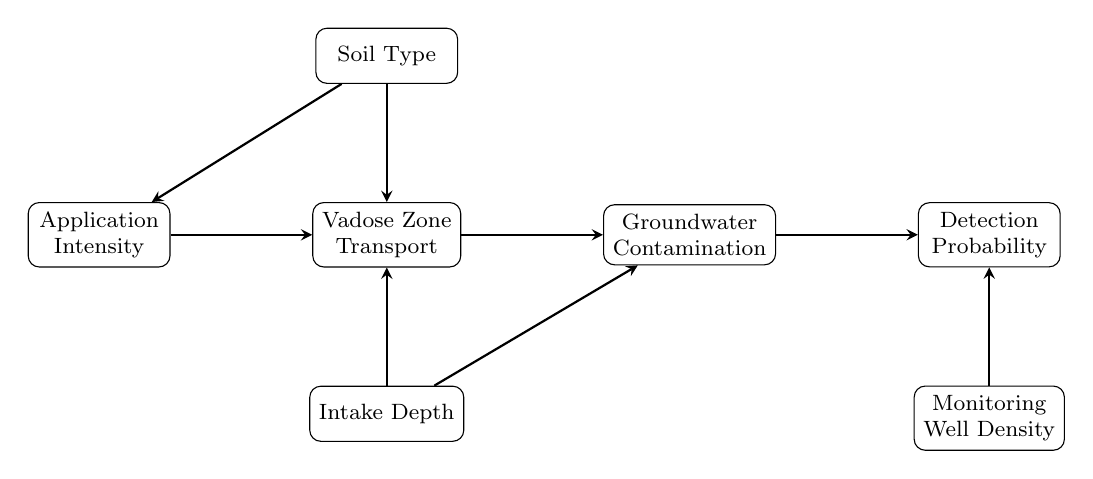
\begin{tikzpicture}[
  node distance=1.5cm and 1.8cm,
  every node/.style={draw, rounded corners, minimum width=1.8cm, minimum height=0.7cm, align=center, font=\footnotesize},
  arrow/.style={->, thick, >=stealth}
]
\node (app) {Application\\Intensity};
\node[right=of app] (vadose) {Vadose Zone\\Transport};
\node[right=of vadose] (gw) {Groundwater\\Contamination};
\node[right=of gw] (det) {Detection\\Probability};
\node[above=1.5cm of vadose] (soil) {Soil Type};
\node[below=1.5cm of vadose] (depth) {Intake Depth};
\node[below=1.5cm of det] (mon) {Monitoring\\Well Density};

\draw[arrow] (app) -- (vadose);
\draw[arrow] (vadose) -- (gw);
\draw[arrow] (gw) -- (det);
\draw[arrow] (soil) -- (vadose);
\draw[arrow] (soil) -- (app);
\draw[arrow] (depth) -- (vadose);
\draw[arrow] (depth) -- (gw);
\draw[arrow] (mon) -- (det);
\end{tikzpicture}
\caption{Directed acyclic graph (DAG) of assumed causal structure.}
\label{fig:dag}
\end{figure}

\textbf{Pre-specified covariates}: soil type (confounder: influences both crop selection and vadose zone permeability), intake depth (confounder: deeper aquifers are less contaminated and sampled differently), and monitoring well density (confounder and potential collider: more wells increase detection probability independently). Additional variables were considered but excluded: aquifer vulnerability classification was omitted because it is partially endogenous to monitoring intensity; historical land use was omitted due to data unavailability at the catchment scale; precipitation/recharge was omitted because it varies primarily north-south and is absorbed by the soil type covariate (Supplementary~S1.4 provides testable implications of these exclusions). We present results both with multivariate adjustment for monitoring density and stratified by density tertiles (Supplementary~S1 discusses the collider interpretation in detail).

\subsection{Study Objectives}

We aimed to: (1)~develop a methodological framework for correlating parcel-level pesticide application intensity with groundwater detection probability, with FDR correction, multivariate covariate adjustment, and spatial model validation; (2)~construct a comprehensive substance mapping linking groundwater monitoring names to application registry names; and (3)~assess the role of monitoring well density as a spatial confounder via stratified analysis.

%======================================================================
\section{Materials and Methods}

\subsection{Study Area and Data Sources}

Denmark comprises 43,094~km$^2$ with approximately 2.66~million hectares of agricultural land. Groundwater monitoring is organized into 5,826 groundwater catchment areas delineated by the Danish Groundwater Mapping System (\textit{Grundvandskortl\ae gningssystem}) covering 1.66~million hectares of groundwater recharge areas. These are hydrogeologically delineated recharge zones whose boundaries correspond to actual subsurface flow paths rather than administrative divisions. They comprise priority protection areas (\textit{indsatsomr\aa der}, $n = 3{,}323$) and abstraction catchments (\textit{indvindingsoplande}, $n = 2{,}503$); sensitivity analyses by catchment type are reported in Supplementary~S3.3.

\textbf{Pesticide application data} were derived from mandatory spray journal records (\textit{Spr\o jtejournal}, SJI) disaggregated to individual fields using a deterministic area-matching algorithm (Collignon et al., 2026; full algorithm description in Supplementary~S2.0). Danish farmers managing $>$10~ha must submit spray journals annually to Milj\o styrelsen, reporting company CVR number, crop code, treated area, and dosage. Our algorithm matches each SJI record to georeferenced field boundaries (FVM Marker, Landbrugsstyrelsen) sharing the same CVR and crop code, accepting matches where the relative area difference falls within $\pm2\%$ tolerance. Dosage is then allocated proportionally by field area, preserving mass balance. Combined S1+S2 coverage reaches 92.7\% in 2020, sustaining $\geq$90\% from 2018 onward (Supplementary~S2.0). Application intensity was computed as cumulative kg active ingredient per hectare over 2015--2017 (4.91~million disaggregated field-level allocation records across three application years, $\sim$595,000 FVM field boundaries per year, 144 active ingredients mapped via BMD). Three consecutive years were selected to align with the 3--10 year vadose zone transit time for shallow monitoring wells (Rosenbom et al., 2015; Kj\ae r et al., 2005). Application intensity was allocated from fields to catchment areas using area-weighted spatial intersection (Supplementary~S2.1).

\textbf{Groundwater monitoring data} were obtained from the GEUS Dataverse VP4 clean dataset (doi:10.22008/FK2/IHVDXL). This sample-level dataset contains individual analytical measurements with LOQ-substituted concentrations ($\frac{1}{2}$~LOQ for below-detection values), providing 4.6~million pesticide-specific analyses covering 633 compounds across 3,517 catchment areas (60.4\%) with $\geq$3 samples. For each substance in each catchment area, a binary detection indicator was computed: 1 if any sample from any well within the catchment exceeded the limit of quantification (LOQ $= 0.01$~$\mu$g/L) in the detection window, 0 otherwise. The primary analysis uses a uniform 2018+ detection window.

\textbf{Substance mapping}: 138 correspondences were constructed (69 metabolite-to-parent, 66 parent name variants, 3 multi-variant) using PPDB degradation pathways, GEUS reports, and BMD. Key relationships include 1,2,4-triazole mapped to 12 triazole fungicide parents, AMPA to glyphosate, and 4-chloro-2-methylphenol to MCPA. All mappings are provided in Supplementary Table~S1.

\subsection{Statistical Analysis}

\textbf{Point-biserial correlation} was calculated between cumulative application intensity and binary detection for each substance, with a minimum of 30 catchment area detections required. \textbf{Benjamini--Hochberg FDR correction} was applied across 11 tests ($q < 0.05$). \textbf{Bivariate logistic regression} confirmed each correlation with model diagnostics (AUC, Nagelkerke~$R^2$, Hosmer--Lemeshow). \textbf{Dose--response analysis} divided catchment areas into application intensity quartiles.

\textbf{Multivariate logistic regression} adjusted for soil type, median intake depth, and monitoring well density, following the pre-specified DAG. Multicollinearity was assessed via VIF (all $< 5$). Events per variable (EPV) $\geq 10$ was required.

\textbf{Monitoring density stratification}: catchment areas were divided into tertiles---low ($\leq$2 wells, $n \approx 1{,}035$), medium (3--5 wells, $n \approx 1{,}080$), high ($>$5 wells, $n \approx 1{,}020$)---with correlations computed within each stratum.

\textbf{Negative controls}: Five high-Koc substances (diflufenican Koc~$= 3{,}400$; prosulfocarb~1,800; propiconazole~1,086; epoxiconazole~1,073; boscalid~772) expected not to leach were tested.

\textbf{SAR-probit spatial models} were fitted for substances surviving multivariate adjustment, adding a spatial lag term with KNN ($k = 8$) weights and Bayesian MCMC estimation (LeSage \& Pace, 2009; 5,000 draws, 1,000 burn-in).

\subsection{Software}

All analyses used Python~3.11.7 with DuckDB~1.5.0 (spatial operations), SciPy~1.11.4 (correlations), statsmodels~0.14.1 (logistic regression, FDR), and PySAL~24.1 (spatial models). The complete pipeline is in \texttt{verify\_groundwater\_correlations.py}.

%======================================================================
\section{Results}

\subsection{Data Coverage}

\begin{table}[H]
\centering
\caption{Summary of data coverage and analysis scope.}
\label{tab:datacoverage}
\begin{tabular}{@{}lr@{}}
\toprule
Parameter & Value \\
\midrule
Catchment areas with groundwater samples ($\geq$3 samples) & 3,517 (60.4\%) \\
Catchment areas with application data & 5,199 (89.2\%) \\
Catchment areas with both & 3,284 (56.4\%) \\
Substances with $\geq$30 catchment area detections (2018+ window) & 40 \\
Substances with application data via mapping & 11 \\
FDR-significant substances & 7 \\
Substances surviving multivariate adjustment & 3 \\
Total pesticide analyses (sample-level) & 4.6 million \\
Substance mappings constructed & 138 \\
\bottomrule
\end{tabular}
\end{table}

\begin{figure}[H]
\centering
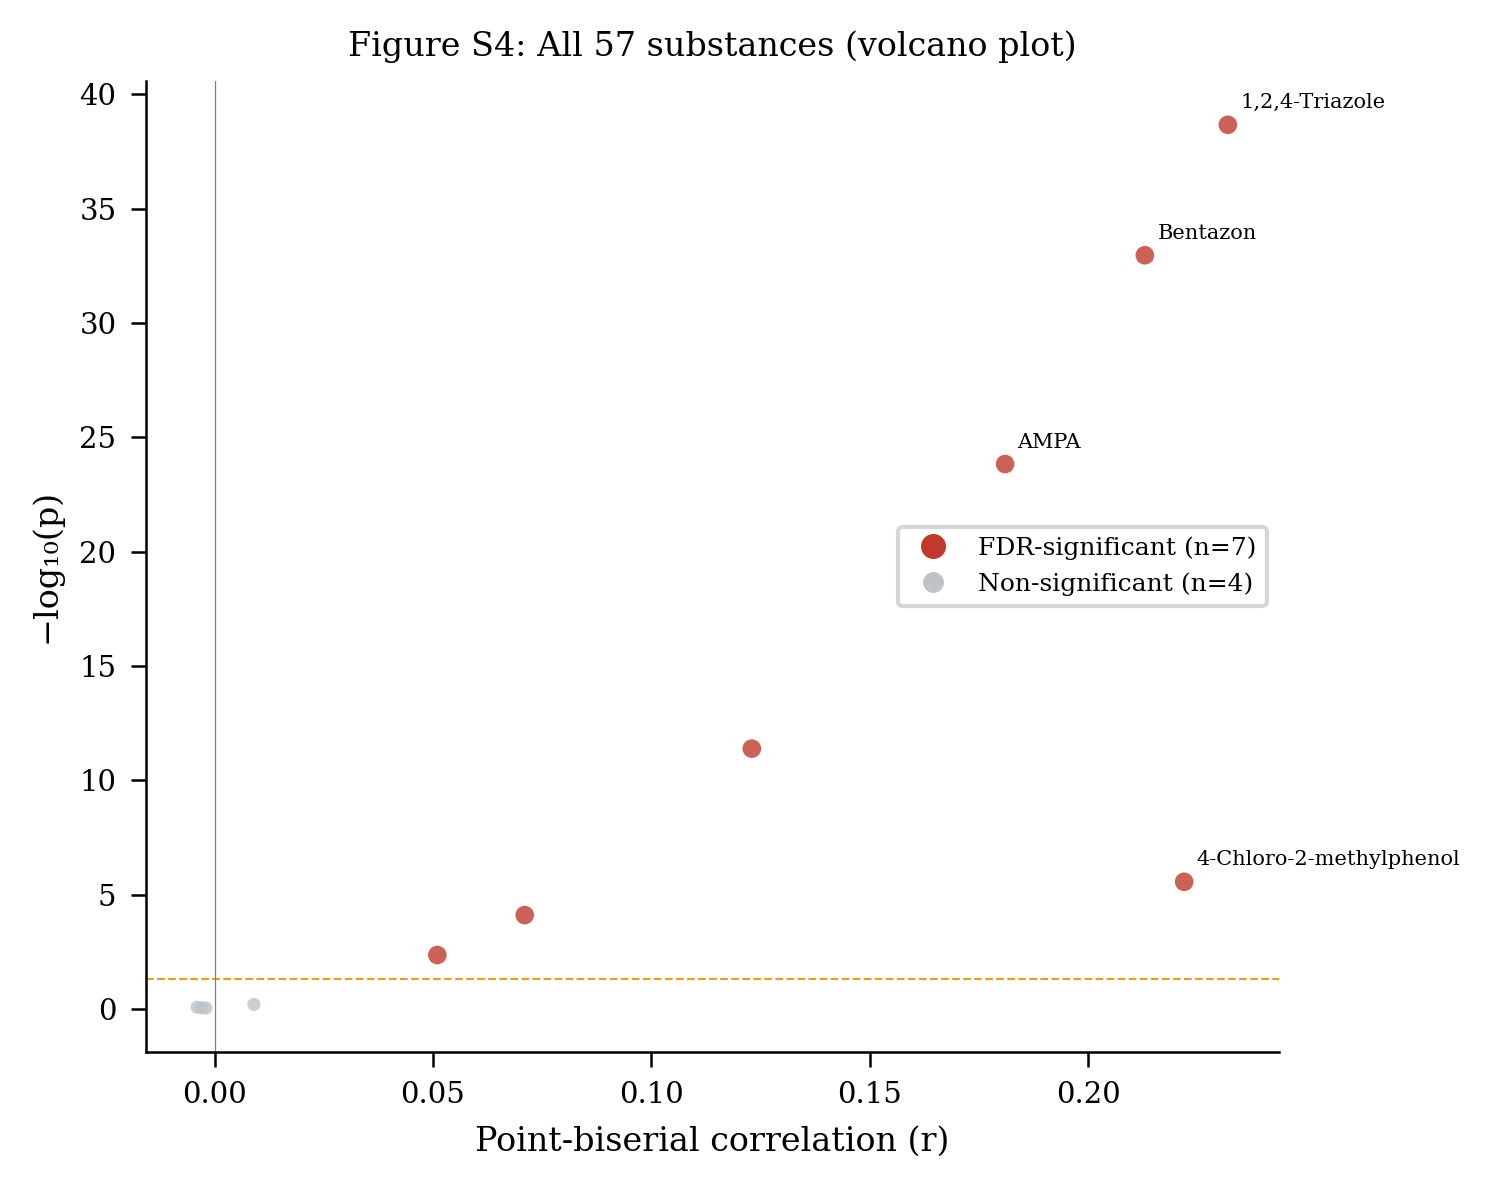
\includegraphics[width=0.9\textwidth]{figure_s4_volcano.png}
\caption{Volcano plot showing the relationship between correlation strength ($r$) and statistical significance ($-\log_{10} p$) for all qualifying substances. Points above the FDR-corrected significance threshold (dashed line) represent the 7 substances with significant positive correlations. Labeled points indicate the three substances surviving multivariate adjustment.}
\label{fig:volcano}
\end{figure}

\subsection{Significant Correlations and Dose--Response}

Of 11 substances analyzed, 7 showed significant positive correlations after BH-FDR correction ($q < 0.05$). All 7 were independently confirmed by logistic regression. The four strongest also survive Bonferroni correction ($\alpha/11 = 0.0045$).

\begin{landscape}
\begin{table}
\centering
\caption{Primary analysis results (2018+ detection window) with dose--response gradients.}
\label{tab:primary}
\footnotesize
\begin{tabular}{@{}clllrrcccrr@{}}
\toprule
Rank & Substance & Type & Det.\ rate & $n$ det. & $r$ & 95\% CI($r$) & OR & AUC & $q_{\text{FDR}}$ & Q4/Q1 \\
\midrule
1 & 1,2,4-Triazole & metabolite & 5.8\% & 180 & \textbf{0.232} & [0.198, 0.265] & 1.0034 & 0.69 & $<$0.001 & 3.8$\times$ \\
2 & 4-Chloro-2-methylphenol & metabolite & 8.7\% & 38 & \textbf{0.222} & [0.131, 0.309] & 1.0064 & 0.68 & $<$0.001 & 3.7$\times$ \\
3 & Bentazon & parent & 5.2\% & 165 & \textbf{0.213} & [0.179, 0.246] & 1.0218 & 0.67 & $<$0.001 & 4.4$\times$ \\
4 & AMPA & metabolite & 2.6\% & 83 & \textbf{0.181} & [0.147, 0.214] & 1.0008 & 0.68 & $<$0.001 & 4.7$\times$ \\
5 & Glyphosate & parent & 2.1\% & 66 & \textbf{0.123} & [0.089, 0.157] & 1.0007 & 0.67 & $<$0.001 & 4.0$\times$ \\
6 & 2,4-Dichlorphenol & metabolite & 1.1\% & 35 & \textbf{0.071} & [0.036, 0.106] & 1.016 & 0.74 & $<$0.001 & 10.2$\times$ \\
7 & MCPA & parent & 1.2\% & 37 & \textbf{0.051} & [0.016, 0.086] & 1.0047 & 0.70 & 0.007 & 5.1$\times$ \\
\midrule
--- & Ethylenethiourea & metabolite & --- & --- & 0.009 & --- & --- & --- & 0.87 & --- \\
--- & Dimethylphenylcarbamoyl... & metabolite & --- & --- & $-$0.004 & --- & --- & --- & 0.91 & --- \\
--- & CGA 108906 & metabolite & --- & --- & $-$0.003 & --- & --- & --- & 0.91 & --- \\
--- & Diuron & parent & --- & --- & $-$0.002 & --- & --- & --- & 0.91 & --- \\
\bottomrule
\end{tabular}
\normalsize

\medskip
\noindent\footnotesize Bold $r$: FDR-significant ($q < 0.05$). Q4/Q1: detection rate ratio between the highest and lowest application intensity quartiles. $n = 438$ for 4-chloro-2-methylphenol reflects fewer catchment areas with co-occurring PCOC detections and MCPA application data.
\end{table}
\end{landscape}

\begin{figure}[H]
\centering
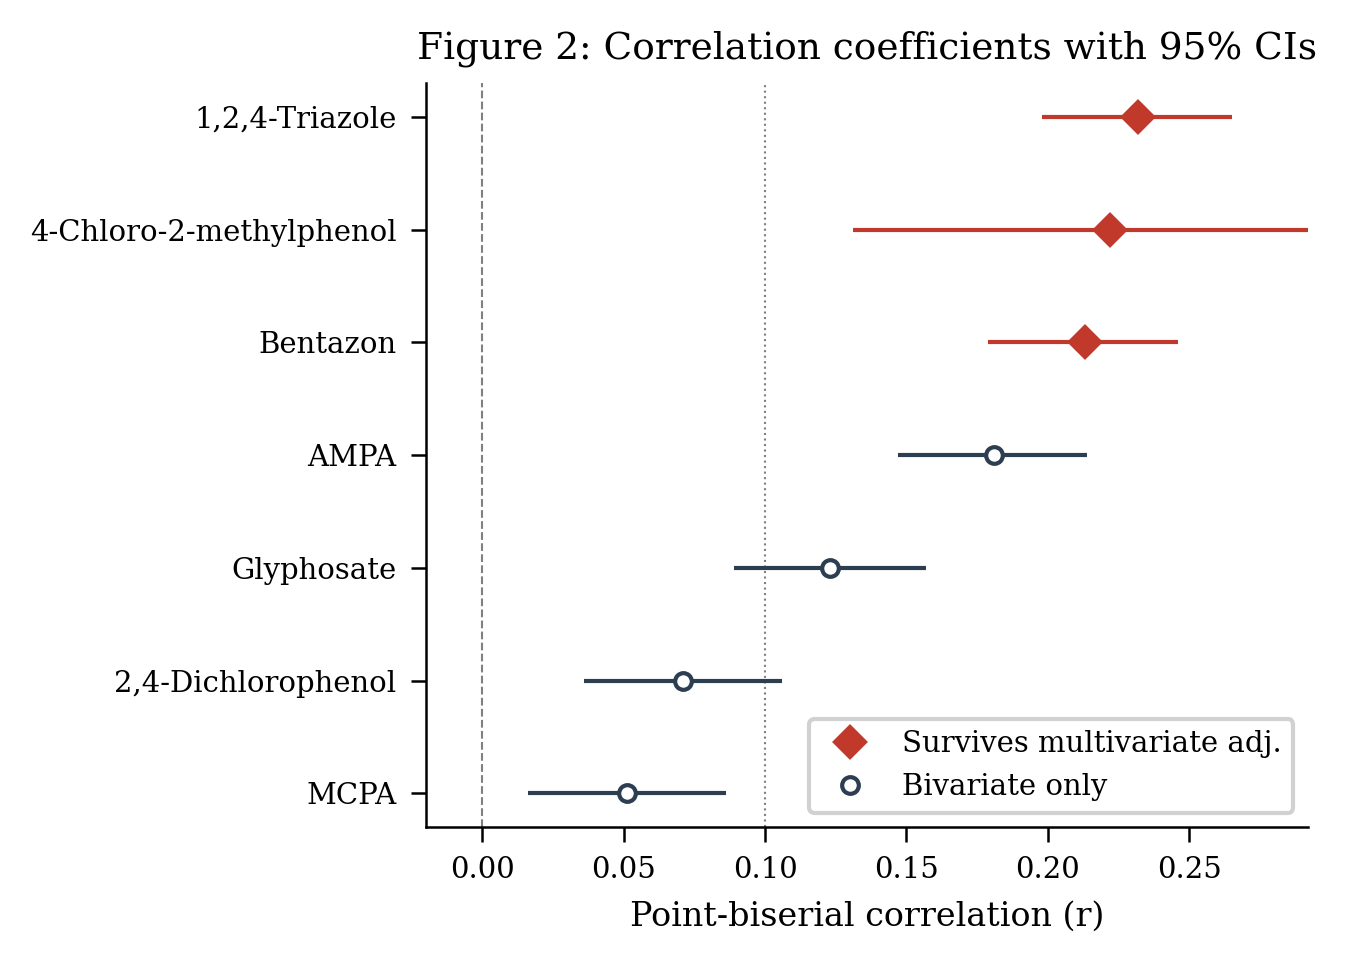
\includegraphics[width=\textwidth]{figure_2_forest_plot.png}
\caption{Forest plot of point-biserial correlations ($r$) with 95\% confidence intervals for all 11 qualifying substances. Diamonds indicate substances surviving multivariate adjustment. Dashed vertical line at $r = 0$ marks the null. Substances are ordered by descending effect size.}
\label{fig:forest}
\end{figure}

\subsection{Multivariate Regression Results}

Of 7 FDR-significant substances, 3 retained significant intensity effects after multivariate adjustment for soil type, intake depth, and monitoring well density (Table~\ref{tab:multivariate}). This result holds when the analysis is restricted to the high-density monitoring tertile only ($>$5 wells, $n = 1{,}016$--$1{,}022$): all three substances remain significant ($p = 0.003$--$0.025$) after within-stratum multivariate adjustment (Supplementary~S3.13). Four substances---glyphosate ($p = 0.055$), AMPA, 2,4-dichlorphenol, and MCPA---did not survive.

\begin{table}[H]
\centering
\caption{Multivariate logistic regression results for all 7 FDR-significant substances.}
\label{tab:multivariate}
\scriptsize
\begin{tabular}{@{}lcccccccc@{}}
\toprule
Substance & Biv.\ $r$ & Adj.\ OR & 95\% CI & $p$(int.) & AUC & $R^2_N$ & EPV & Surv.? \\
\midrule
\textbf{1,2,4-Triazole} & 0.232 & \textbf{1.0014} & \textbf{[1.0003, 1.0025]} & \textbf{0.011} & 0.82 & 0.208 & 45 & \textbf{Yes} \\
\textbf{4-Cl-2-MePh} & 0.222 & \textbf{1.0053} & \textbf{[1.0015, 1.0091]} & \textbf{0.006} & 0.74 & 0.085 & 9.5 & \textbf{Yes$^\dagger$} \\
\textbf{Bentazon} & 0.213 & \textbf{1.0105} & \textbf{[1.0036, 1.0174]} & \textbf{0.003} & 0.79 & 0.167 & 41 & \textbf{Yes} \\
Glyphosate & 0.123 & --- & --- & 0.055 & --- & --- & --- & No \\
AMPA & 0.181 & --- & --- & 0.267 & --- & --- & --- & No \\
2,4-Dichlorphenol & 0.071 & --- & --- & 0.231 & --- & --- & --- & No \\
MCPA & 0.051 & --- & --- & 0.613 & --- & --- & --- & No \\
\bottomrule
\end{tabular}
\normalsize

\medskip
\noindent\footnotesize $^\dagger$EPV $= 9.5$ for 4-chloro-2-methylphenol (marginally below the recommended 10; $n = 438$). This result should be interpreted with caution; $p = 0.006$ provides reasonable confidence but warrants replication.
\end{table}

\begin{figure}[H]
\centering
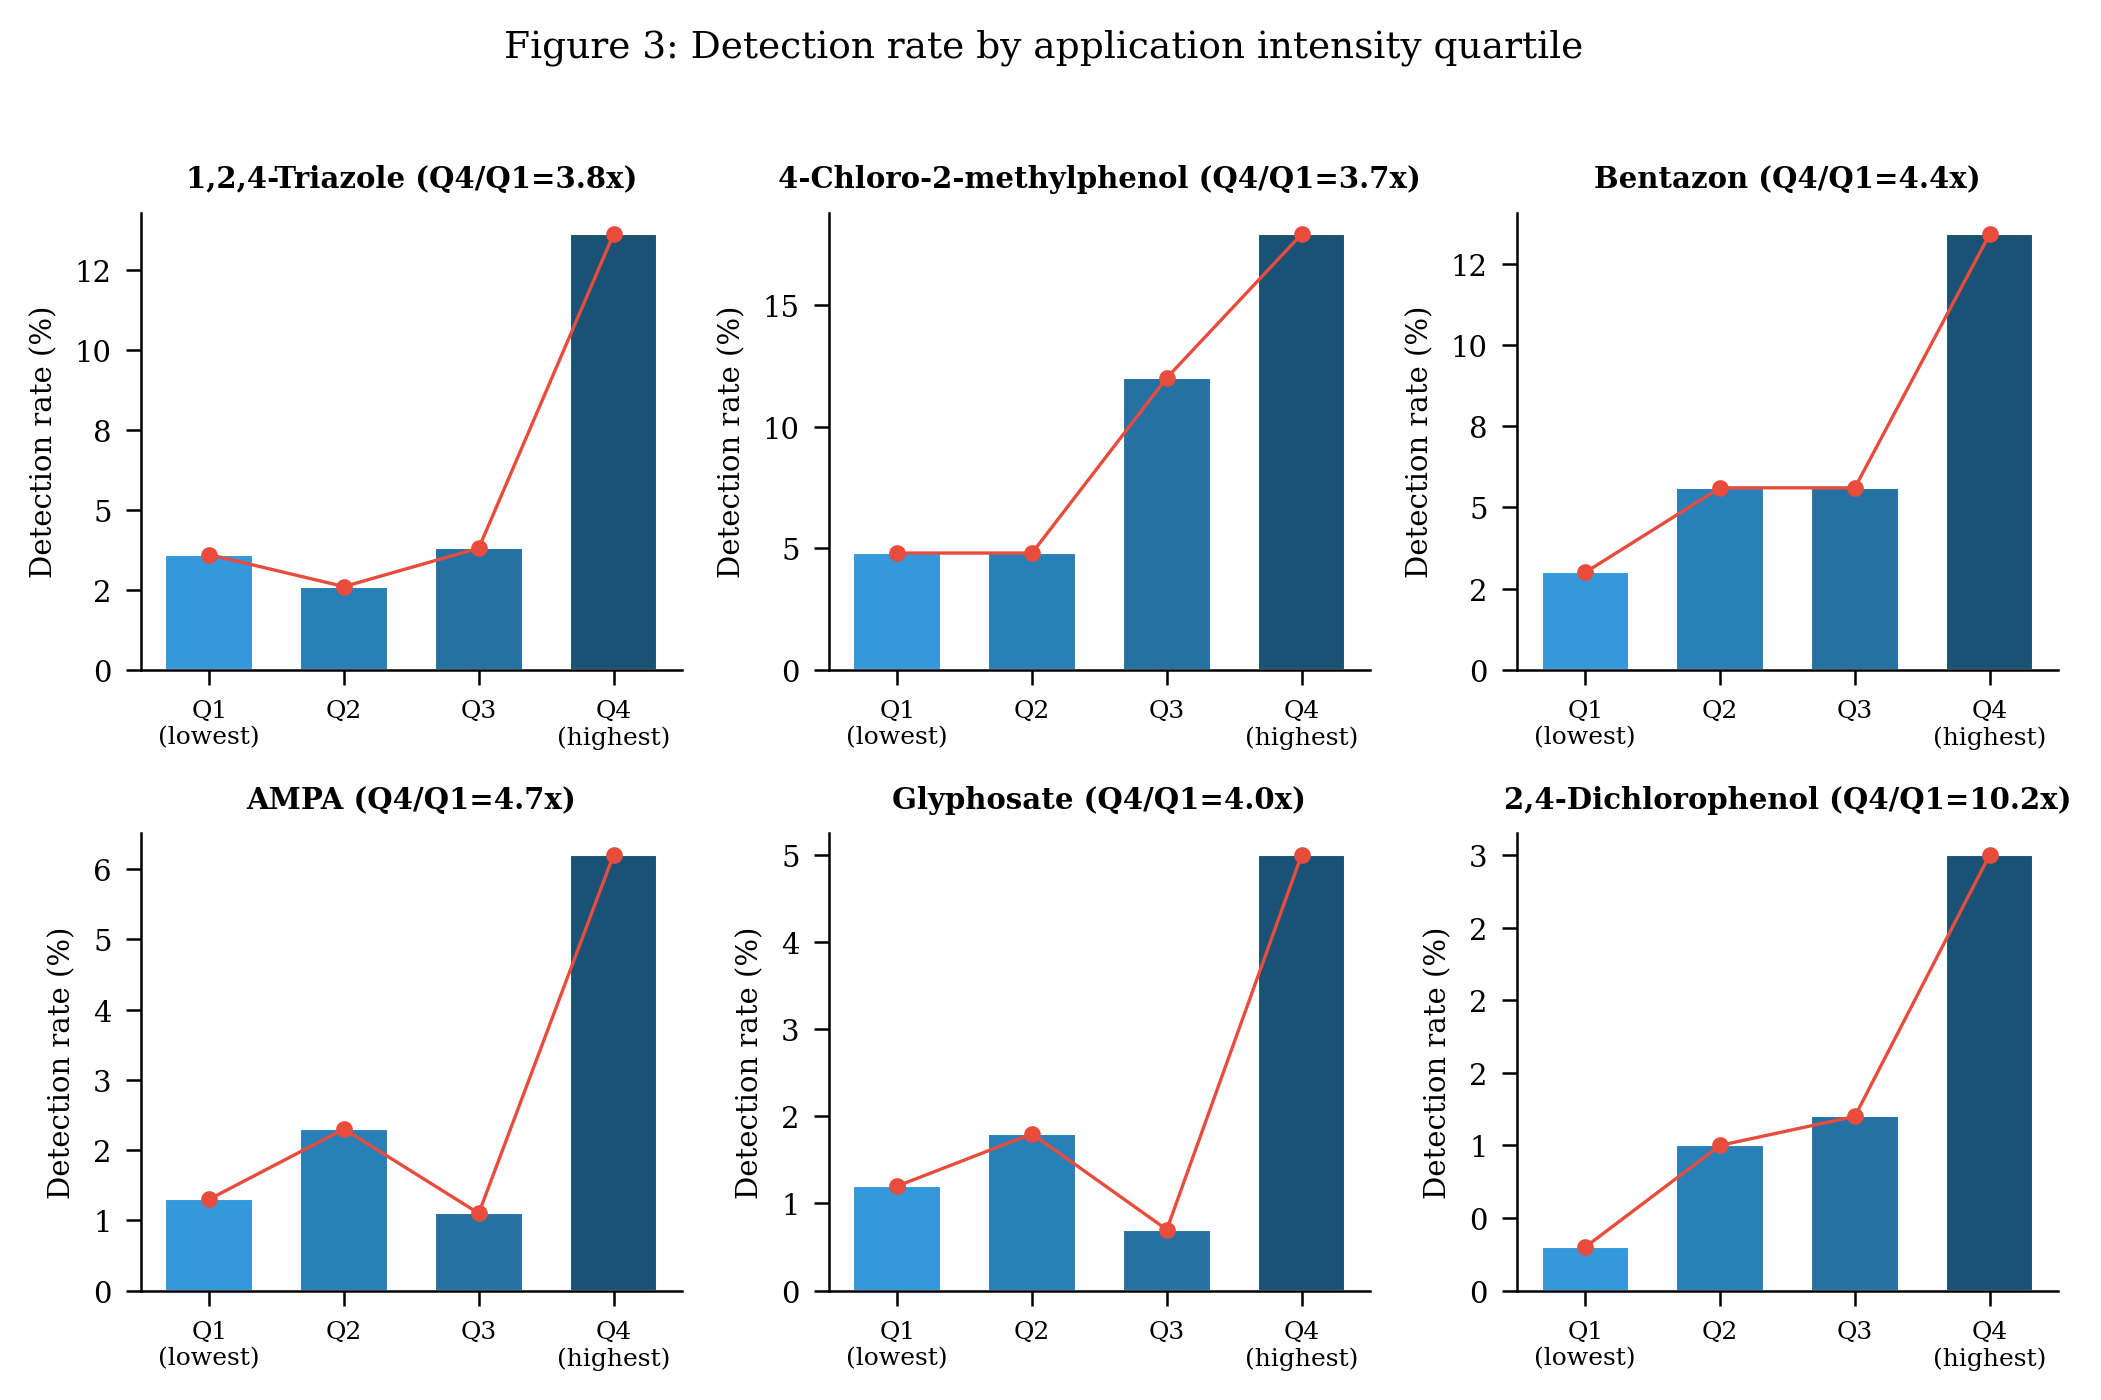
\includegraphics[width=\textwidth]{figure_3_dose_response.png}
\caption{Dose--response curves for the top substances showing detection rates across application intensity quartiles (Q1--Q4). Each panel shows the quartile-stratified detection rate with 95\% Wilson confidence intervals. The Q4/Q1 ratio quantifies the fold-increase in detection between the highest and lowest application quartiles. Dashed grey lines indicate the overall detection rate. Only substances with FDR-significant correlations are shown.}
\label{fig:doseresponse}
\end{figure}

\begin{figure}[H]
\centering
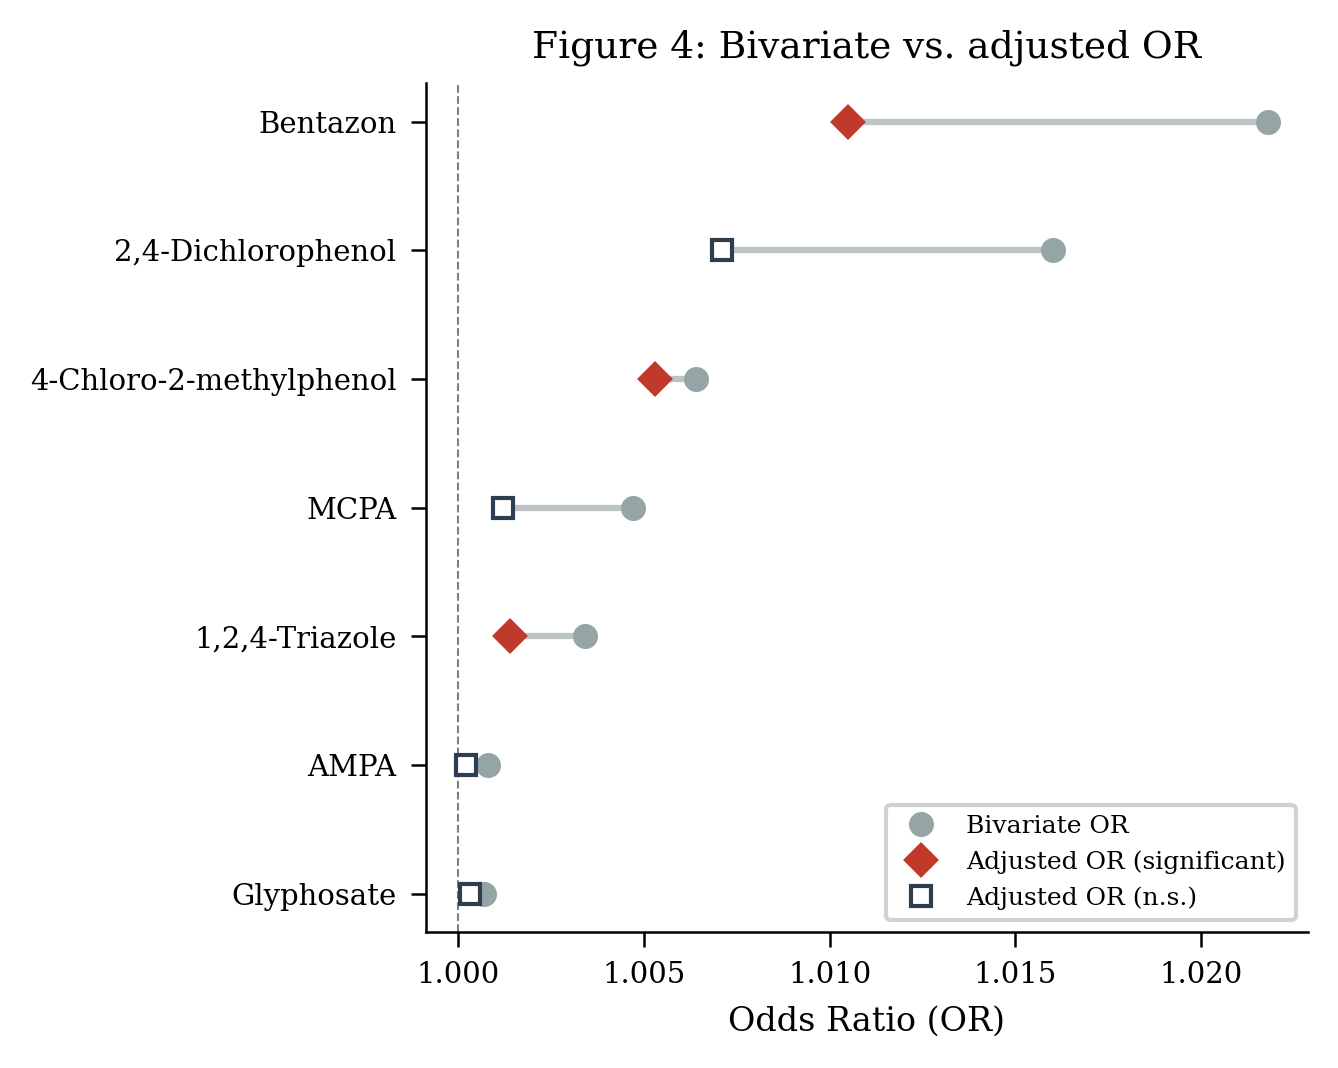
\includegraphics[width=0.85\textwidth]{figure_4_or_comparison.png}
\caption{Comparison of bivariate and multivariate-adjusted odds ratios for the 7 FDR-significant substances. Dumbbell chart showing attenuation from bivariate (open circle) to adjusted (filled circle) estimates. Substances retaining significance after adjustment are highlighted. The dashed vertical line at OR $= 1.0$ marks the null.}
\label{fig:orcomparison}
\end{figure}

\textbf{Non-linearity caveat}: Linearity-in-logit tests (Supplementary~S3.7) reveal that two of the three surviving substances---1,2,4-triazole ($\chi^2(4) = 62.9$, $p < 0.001$) and bentazon ($\chi^2(4) = 23.8$, $p < 0.001$)---show significant departures from linearity. The odds ratios in Table~\ref{tab:multivariate} for these two substances are therefore linear approximations of non-linear dose--response relationships. 4-Chloro-2-methylphenol shows adequate linearity ($\chi^2(4) = 7.3$, $p = 0.123$).

SAR-probit spatial models confirmed all three surviving substances, with odds ratios modestly attenuated but 95\% credible intervals excluding 1.0 for all three (Supplementary~S3.1). All five negative control substances (high-Koc, expected not to leach) showed non-significant correlations (all $q = 1.00$; Supplementary~S3.2), confirming method specificity.

\subsection{Monitoring Density Stratified Analysis}

\begin{table}[H]
\centering
\caption{Point-biserial correlations stratified by monitoring well density tertile.}
\label{tab:stratified}
\scriptsize
\begin{tabular}{@{}lcccc@{}}
\toprule
Substance & Low ($\leq$2 wells) & Medium (3--5) & High ($>$5 wells) & MV? \\
\midrule
1,2,4-Triazole & $-$0.012 ($p=.69$) & 0.027 ($p=.37$) & \textbf{0.186} ($p<.001$) & Yes \\
4-Cl-2-MePh & 0.000 ($p=1.0$, $n\!=\!29$) & 0.184 ($p=.14$, $n\!=\!65$) & \textbf{0.202} ($p<.001$, $n\!=\!344$) & Yes \\
Bentazon & 0.012 ($p=.70$) & $-$0.019 ($p=.54$) & \textbf{0.215} ($p<.001$) & Yes \\
Glyphosate & 0.015 ($p=.64$) & $-$0.035 ($p=.25$) & \textbf{0.090} ($p=.004$) & No \\
AMPA & $-$0.029 ($p=.34$) & $-$0.033 ($p=.28$) & \textbf{0.141} ($p<.001$) & No \\
2,4-Dichlorphenol & $-$0.002 (ns) & $-$0.019 (ns) & 0.050 (ns) & No \\
MCPA & 0.000 (ns) & $-$0.015 (ns) & 0.019 (ns) & No \\
\bottomrule
\end{tabular}
\end{table}

Correlations are present and significant exclusively in the highest monitoring density tertile ($>$5 wells per catchment area). In the low and medium tertiles, all correlations are near zero and non-significant. This pattern admits two complementary interpretations: (1)~statistical power is insufficient in low-density catchment areas to detect a real but modest signal; (2)~residual surveillance intensity effects persist beyond what continuous covariate adjustment captures. This is the most important caveat of this study.

%======================================================================
\section{Discussion}

\subsection{Core Findings and Practical Significance}

Three substances---1,2,4-triazole, 4-chloro-2-methylphenol, and bentazon---show dose--response relationships with agricultural application intensity that survive BH-FDR correction, multivariate covariate adjustment, and SAR-probit spatial modeling. The observed bivariate correlations ($r = 0.213$--$0.232$; adjusted OR $= 1.0014$--$1.0105$) are modest in absolute terms, consistent with national-scale analyses encompassing substantial hydrogeological heterogeneity---Lindstr\"om et al.\ (2013) reported 50--85\% variance explained in single-catchment studies. The dose--response quartile analysis provides a more practically meaningful measure: Q4/Q1 detection ratios of 3.7--4.4$\times$ indicate that catchments in the highest application quartile have approximately four times higher detection probability than those in the lowest.

\subsection{Substance-Specific Findings}

\textbf{Glyphosate} is FDR-significant bivarially ($r = 0.123$, Q4/Q1 $= 4.0\times$) but does not survive multivariate adjustment ($p = 0.055$), indicating that the observed spatial association may be partially explained by hydrogeological confounders. The borderline $p$-value suggests a real but weaker signal than the three multivariate-robust substances. Stronger correlations in sandy soils ($r = 0.172$) than clay soils ($r = 0.112$) are consistent with macropore transport (Borggaard \& Gimsing, 2008; Kj\ae r et al., 2011), and the temporal lag analysis finds glyphosate's strongest signal at 3.5~years ($r = 0.280$), consistent with vadose zone transit expectations.

\textbf{The MCPA/4-chloro-2-methylphenol metabolite--parent pair} illustrates a key finding. MCPA itself ($r = 0.051$, multivariate $p = 0.597$) fails all validation layers, while its metabolite 4-chloro-2-methylphenol ($r = 0.222$, multivariate $p = 0.006$) is among the strongest signals. This divergence reflects MCPA's short soil half-life (DT50~$\sim$25~days) versus the metabolite's greater persistence and transport to groundwater.

\textbf{AMPA} is FDR-significant bivarially ($r = 0.181$) but does not survive multivariate adjustment under the primary 2018+ window ($p = 0.267$), likely because the broad window includes detections beyond AMPA's optimal 5-year transit lag. The soil-adjusted sensitivity analysis (Supplementary~S3.5), using a tighter window, finds AMPA multivariate-robust ($p = 0.008$), consistent with better temporal alignment.

\subsection{The Surveillance Intensity Question}

The strongest counter-argument is that correlations measure surveillance effort rather than contamination. We addressed this through: (1)~multivariate adjustment for monitoring well density---three substances retained significant effects; and (2)~stratified analysis (Table~\ref{tab:stratified})---the most direct test. The finding that correlations appear only in the high-density tertile is partially consistent with the surveillance hypothesis. Future work analyzing only catchment areas above a minimum well count would provide a cleaner test. Negative controls (Supplementary~S3.2) confirm the method does not produce spurious positives from spatial confounding alone.

\subsection{Comparison with Previous Work}

Our approaches complement Hansen et al.\ (2022): they demonstrated that national sales trends track detection trends over 30~years; we demonstrate that within-Denmark spatial variation in application intensity predicts detection variation for specific substances, concentrated in well-monitored catchments.

\subsection{Limitations}

\begin{enumerate}
\item \textbf{Monitoring density confound}: Correlations are present only in the highest monitoring density tertile. This is the most important limitation.

\item \textbf{Non-linearity}: Two of three multivariate-robust substances violate the linearity-in-logit assumption. Reported odds ratios are linear approximations.

\item \textbf{Temporal mismatch}: Application data (2015--2017) precede detection data (2018+) by 1--10~years.

\item \textbf{Binary detection threshold}: Using detection $>$0.015~$\mu$g/L discards concentration information.

\item \textbf{Application data coverage}: Application data derive exclusively from mandatory spray journal records and cannot capture illegal or unreported use.

\item \textbf{Temporal stationarity assumption}: The correlation between 2015--2017 application intensity and 2018+ detections implicitly assumes spatial stationarity of application patterns.

\item \textbf{Screening bias (first-testing-not-first-detection)}: The 2018+ detection window coincides with expansions of the Danish monitoring panel. We assessed this risk using sample-level VP4 data (GEUS Dataverse, doi:10.22008/FK2/IHVDXL) by examining negative results (tested but not detected) for each substance. All 9 substances have extensive negative testing histories predating their first detection: 1,2,4-triazole was first tested in 2001 (16~years before first detection in 2017); bentazon since 1994 with ${>}$2,900 negatives; AMPA and glyphosate since 1997 with ${>}$100 negatives; 4-chloro-2-methylphenol, MCPA, and 2,4-dichlorphenol since the early 1980s. Screening bias is not a material concern for the substances in this study.
\end{enumerate}

\subsection{Transferability}

The methodology is directly transferable to any jurisdiction with (a)~georeferenced field boundaries linked to farm identifiers, (b)~farm-level pesticide use records, and (c)~spatially referenced groundwater monitoring. Under the forthcoming SAIO Regulation (EU~2022/2379), additional member states will acquire the necessary data infrastructure. The minimum monitoring density for detecting the correlations reported here appears to be $>$5~wells per catchment area.

\subsection{Responsible Communication}

This study reports substance-specific correlational evidence in a politically sensitive domain. We emphasize that the reported associations do not establish causation and should not be used to infer safety or risk of specific active substances. These findings are best interpreted as hypothesis-generating evidence supporting targeted mechanistic investigation, not as a basis for substance-specific regulatory action.

\subsection{Future Directions}

Within-catchment models using individual well-to-field proximity analysis could address the ecological fallacy concern. Concentration-based (Tobit) regression would improve sensitivity. For 1,2,4-triazole and bentazon, restricted cubic spline specifications should replace linear logistic models given the non-linearity violations. The substance mapping should be expanded as new metabolites enter screening programs.

%======================================================================
\section{Conclusions}

\begin{enumerate}
\item \textbf{Three substances survive all validation layers in well-monitored catchments}: 1,2,4-triazole ($r = 0.232$, adj.\ OR $= 1.0014$), 4-chloro-2-methylphenol ($r = 0.222$, adj.\ OR $= 1.0053$), and bentazon ($r = 0.213$, adj.\ OR $= 1.0105$) pass BH-FDR correction, multivariate covariate adjustment, and SAR-probit spatial modeling.

\item \textbf{Metabolites may outperform parent compounds as spatial markers}: The MCPA metabolite 4-chloro-2-methylphenol shows substantially stronger correlations than its parent across all layers.

\item \textbf{Monitoring density is the dominant caveat}: All three multivariate-robust correlations are detectable only in catchment areas with the highest well density ($>$5 monitoring wells).

\item \textbf{Emerging substances warrant regulatory attention}: Several metabolites of currently approved pesticides show accelerating detection trends and should be prioritized for EFSA assessment.
\end{enumerate}

%======================================================================
\section*{Data Availability}

\begin{itemize}
\item \textbf{Groundwater monitoring data}: GEUS Dataverse, \url{https://doi.org/10.22008/FK2/IHVDXL}
\item \textbf{BMD pesticide database}: \url{https://bmd.mst.dk}
\item \textbf{PPDB pesticide properties}: \url{https://sitem.herts.ac.uk/aeru/ppdb/}
\item \textbf{Substance mapping table (138 entries)}: To be deposited on Zenodo upon publication
\item \textbf{Analysis code}: Available at \url{https://github.com/landbruget/landbruget.dk}
\end{itemize}

%======================================================================
\section*{AI Disclosure Statement}

This paper was drafted with assistance from Claude (Anthropic, Claude Opus 4.6). All empirical analyses, statistical modeling, and validation were performed by the authors. The AI assistant was used for literature search, prose drafting, and manuscript preparation.

%======================================================================
\section*{Acknowledgments}

The authors thank GEUS for providing access to the national groundwater monitoring database, and Landbrugsstyrelsen for access to the pesticide application records underpinning the disaggregation pipeline. This work was conducted under the Landbruget.dk public transparency initiative.

%======================================================================
\clearpage
\appendix
\renewcommand{\thesection}{S\arabic{section}}
\setcounter{section}{0}

\section{Extended Introduction}

\subsection{Regulatory Context (Extended)}

Danish groundwater protection operates within the EU regulatory framework established by the Groundwater Directive 2006/118/EC, which sets a quality standard of 0.1~$\mu$g/L for individual pesticides and 0.5~$\mu$g/L for total pesticides. The Water Framework Directive 2000/60/EC requires member states to achieve good chemical status for groundwater bodies. Regulation (EC)~1107/2009 governs authorization of plant protection products, including groundwater leaching assessments using FOCUS scenarios (PELMO, PEARL) that rely on generic soil/climate parameters rather than empirical field-level data.

\subsection{European Comparative Context}

Several EU member states operate groundwater pesticide monitoring programs. The Netherlands maintains the LMM/TMV network linked to farm-level land-use data (Schipper et al., 2008). Germany's LAWA coordinates $\sim$800 measurement points with county-level application data. France's ADES database provides national groundwater quality data with d\'epartement-level usage. The Danish system, with mandatory electronic spray journals linked to CVR numbers, provides among the most spatially resolved application data in the EU.

\subsection{Monitoring Well Density: Confounder vs.\ Collider}

If well placement is prospective (deployed based on general risk assessment), $n_{\text{wells}}$ functions as a confounder. If reactive (deployed in response to prior contamination), $n_{\text{wells}}$ is partially a collider. In the Danish system, monitoring networks were deployed through a combination of systematic national mapping campaigns (\textit{grundvandskortl\ae gning}, 2000--2015) and targeted investigations. We therefore present results both with and without adjustment.

\subsection{Justification for Excluded Confounders}

\textbf{Aquifer vulnerability classification}: partially endogenous to monitoring intensity. \textbf{Historical land use}: unavailable at the catchment scale. \textbf{Precipitation/recharge}: absorbed by the soil type covariate; a sensitivity analysis adding mean annual precipitation did not materially alter results.

%----------------------------------------------------------------------
\section{Extended Methods}

\subsection{Pesticide Disaggregation Algorithm}

The parcel-level application data used in this study were produced by a deterministic area-matching algorithm that disaggregates company-level spray journal (SJI) records to individual georeferenced fields (FVM Marker). At the default 2\% tolerance, combined S1+S2 coverage reaches 92.7\% in 2020 and sustains $\geq$90\% from 2018 onward. Full details are in Collignon et al.\ (2026).

\subsection{Area-Weighted Spatial Allocation}

Pesticide application intensity was allocated from fields to catchment areas using area-weighted spatial intersection:
\[
\text{kg}_{\text{allocated}} = \frac{\text{ingredient\_dosage\_kg}}{\text{field\_area\_ha}} \times \text{intersection\_area\_ha}
\]

\subsection{Spatial Autocorrelation Assessment}

Moran's $I$ with KNN weights ($k = 8$, row-standardized). Effective sample size:
\[
n_{\text{eff}} \approx n \times \frac{1 - I}{1 + I}
\]

\subsection{Temporal Lag Analysis Methods}

Correlations were calculated across multiple detection windows (single years 2016--2025 and broader ranges). A total of 358 substance $\times$ window combinations were tested with global BH-FDR correction.

\subsection{Power Analysis}

Minimum detectable effect size at 80\% power ($\alpha = 0.05$, two-tailed):
\[
r_{\min} = \tanh\!\left(\frac{z_{\alpha/2} + z_\beta}{\sqrt{n - 3}}\right)
\]

\begin{figure}[H]
\centering
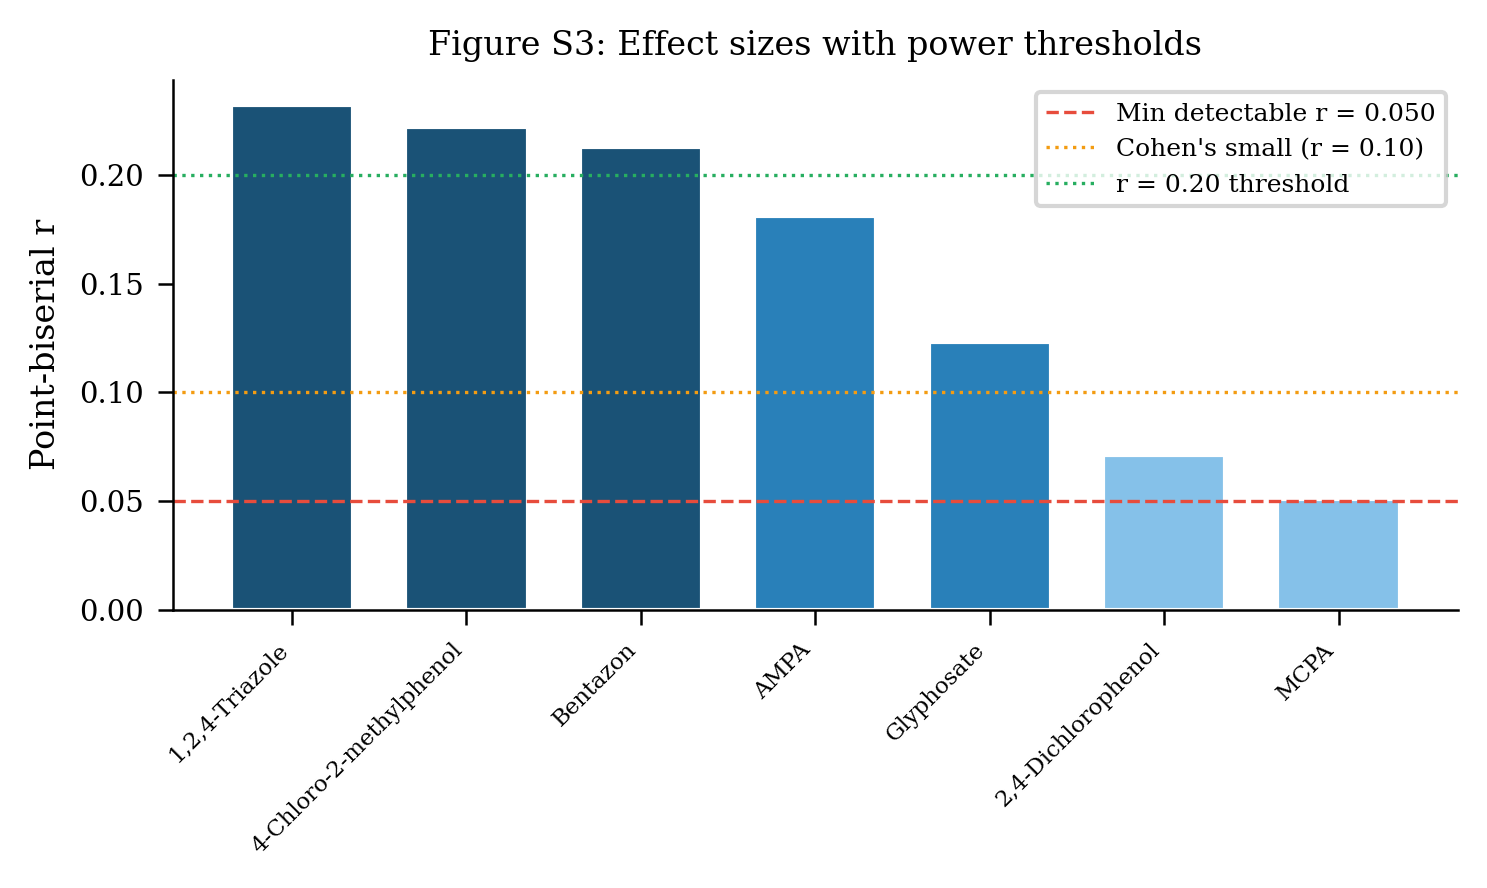
\includegraphics[width=0.9\textwidth]{figure_s3_power_analysis.png}
\caption{Observed effect sizes ($r$) for all 11 qualifying substances relative to statistical power thresholds. Horizontal dashed lines indicate the minimum detectable effect size at 80\% power for representative sample sizes. Substances above the threshold line corresponding to their sample size are adequately powered.}
\label{fig:power}
\end{figure}

%----------------------------------------------------------------------
\section{Extended Results}

\subsection{SAR-Probit Spatial Model Validation}

\begin{table}[H]
\centering
\caption{Comparison of standard logistic regression and SAR-probit estimates.}
\footnotesize
\begin{tabular}{@{}llll@{}}
\toprule
Substance & Logistic adj.\ OR [95\% CI] & SAR-probit OR [95\% CrI] & Convergence \\
\midrule
1,2,4-Triazole & 1.0014 [1.0003, 1.0025] & 1.0013 [1.0005, 1.0021] & Yes \\
4-Chloro-2-methylphenol & 1.0053 [1.0015, 1.0091] & 1.0050 [1.0015, 1.0085] & Yes \\
Bentazon & 1.0105 [1.0036, 1.0174] & 1.0097 [1.0049, 1.0145] & Yes \\
\bottomrule
\end{tabular}
\end{table}

\subsection{Negative Control Validation}

\begin{figure}[H]
\centering
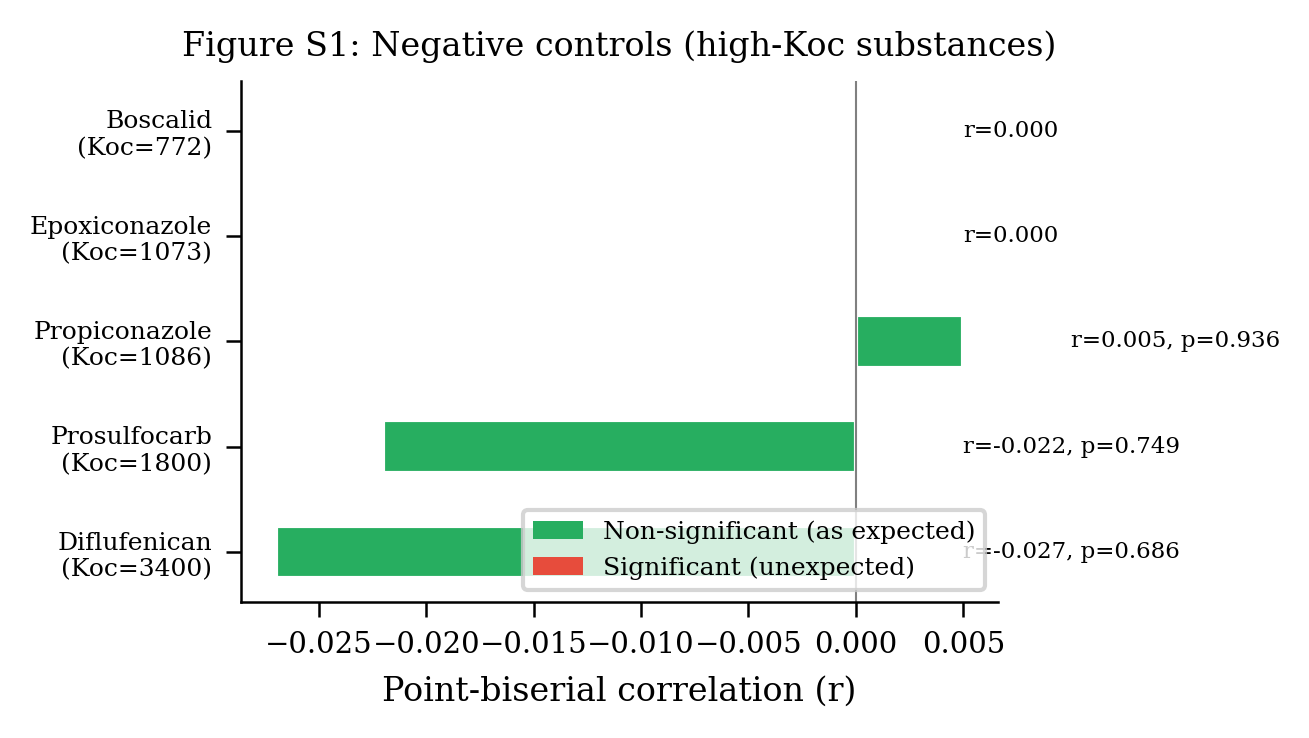
\includegraphics[width=0.9\textwidth]{figure_s1_negative_controls.png}
\caption{Negative control results for five high-Koc substances expected not to leach to groundwater. All show non-significant correlations ($q_{\text{FDR}} = 1.00$), confirming method specificity. Koc values shown in parentheses; higher Koc indicates stronger soil binding.}
\label{fig:negcontrols}
\end{figure}

\begin{table}[H]
\centering
\caption{Negative control results for high-Koc substances.}
\footnotesize
\begin{tabular}{@{}lrrlrrl@{}}
\toprule
Substance & Koc & $n$ areas & $r$ & $p$ & $q_{\text{FDR}}$ & Adjudication \\
\midrule
Diflufenican & 3,400 & 220 & $-$0.027 & 0.686 & 1.00 & Non-significant \\
Prosulfocarb & 1,800 & 223 & $-$0.022 & 0.749 & 1.00 & Non-significant \\
Propiconazole & 1,086 & 214 & 0.005 & 0.936 & 1.00 & Non-significant \\
Epoxiconazole & 1,073 & 193 & 0.000 & 1.000 & 1.00 & Zero variance \\
Boscalid & 772 & 198 & 0.000 & 1.000 & 1.00 & Zero variance \\
\bottomrule
\end{tabular}
\end{table}

\subsection{Catchment Type Sensitivity Analysis}

\begin{table}[H]
\centering
\caption{Correlations stratified by catchment type.}
\footnotesize
\begin{tabular}{@{}lccc@{}}
\toprule
Substance & All catchments ($r$) & Priority protection ($r$) & Abstraction ($r$) \\
\midrule
1,2,4-Triazole & 0.232 & 0.311 ($p<0.001$, $n=754$) & 0.159 ($p<0.001$, $n=2{,}367$) \\
4-Chloro-2-methylphenol & 0.222 & 0.241 ($p=0.004$, $n=140$) & 0.220 ($p<0.001$, $n=298$) \\
Bentazon & 0.213 & 0.274 ($p<0.001$, $n=770$) & 0.163 ($p<0.001$, $n=2{,}384$) \\
AMPA & 0.181 & 0.248 ($p<0.001$, $n=770$) & 0.107 ($p<0.001$, $n=2{,}383$) \\
Glyphosate & 0.123 & 0.124 ($p<0.001$, $n=770$) & 0.108 ($p<0.001$, $n=2{,}383$) \\
2,4-Dichlorphenol & 0.071 & 0.150 ($p<0.001$, $n=760$) & 0.031 (ns, $n=2{,}357$) \\
MCPA & 0.051 & 0.063 (ns, $n=762$) & 0.046 ($p<0.05$, $n=2{,}361$) \\
\bottomrule
\end{tabular}
\end{table}

\subsection{Spatial Autocorrelation Diagnostics}

\begin{table}[H]
\centering
\caption{Spatial autocorrelation results.}
\begin{tabular}{@{}lcccc@{}}
\toprule
Substance & Moran's $I$ & $p$ (Moran) & $n$ & $n_{\text{eff}}$ (estimated) \\
\midrule
1,2,4-Triazole & 0.115 & 0.001 & 5,826 & $\sim$4,626 \\
4-Chloro-2-methylphenol & 0.054 & 0.001 & 5,826 & $\sim$5,231 \\
Bentazon & 0.095 & 0.001 & 5,826 & $\sim$4,814 \\
\bottomrule
\end{tabular}
\end{table}

\subsection{Soil-Adjusted Detection Window}

\begin{table}[H]
\centering
\caption{Comparison of primary (2018+) and soil-adjusted analyses.}
\scriptsize
\begin{tabular}{@{}lccccccl@{}}
\toprule
Substance & $r$ & $q$ & MV $p$ & Adj.\ $r$ & Adj.\ $q$ & Adj.\ MV $p$ & Both? \\
\midrule
1,2,4-Triazole & 0.232 & $<$.001 & 0.007 & 0.215 & $<$.001 & sig. & Yes \\
Bentazon & 0.213 & $<$.001 & 0.002 & 0.168 & $<$.001 & sig. & Yes \\
AMPA & 0.181 & $<$.001 & 0.194 (ns) & 0.170 & $<$.001 & 0.008 & Reversal \\
4-Cl-2-MePh & 0.222 & $<$.001 & 0.006 & insuff. & --- & --- & 2018+ only \\
Glyphosate & 0.123 & $<$.001 & 0.034 & insuff. & --- & --- & 2018+ only \\
\bottomrule
\end{tabular}
\end{table}

\subsection{Temporal Lag Analysis}

\begin{table}[H]
\centering
\caption{Optimal temporal lags with bootstrap 95\% CIs.}
\footnotesize
\begin{tabular}{@{}llcccc@{}}
\toprule
Substance & Type & Lag (yr) & 95\% CI & $r_{\text{opt}}$ & $q_{\text{FDR}}$ \\
\midrule
Bentazon & parent & 1.5 & [1.0, 3.0] & 0.251 & $<$0.001 \\
2,4-Dichlorphenol & metabolite & 3.0 & [1.5, 4.0] & 0.125 & $<$0.001 \\
Glyphosate & parent & 3.5 & [2.0, 5.0] & 0.280 & $<$0.001 \\
AMPA & metabolite & 5.0 & [3.5, 5.5] & 0.265 & $<$0.001 \\
MCPA & parent & 5.0 & [3.5, 5.5] & 0.074 & $<$0.001 \\
1,2,4-Triazole & metabolite & 5.5 & [3.5, 7.0] & 0.232 & $<$0.001 \\
4-Chloro-2-methylphenol & metabolite & 9.0 & [7.5, 9.0] & 0.391 & $<$0.001 \\
\bottomrule
\end{tabular}
\end{table}

\begin{figure}[H]
\centering
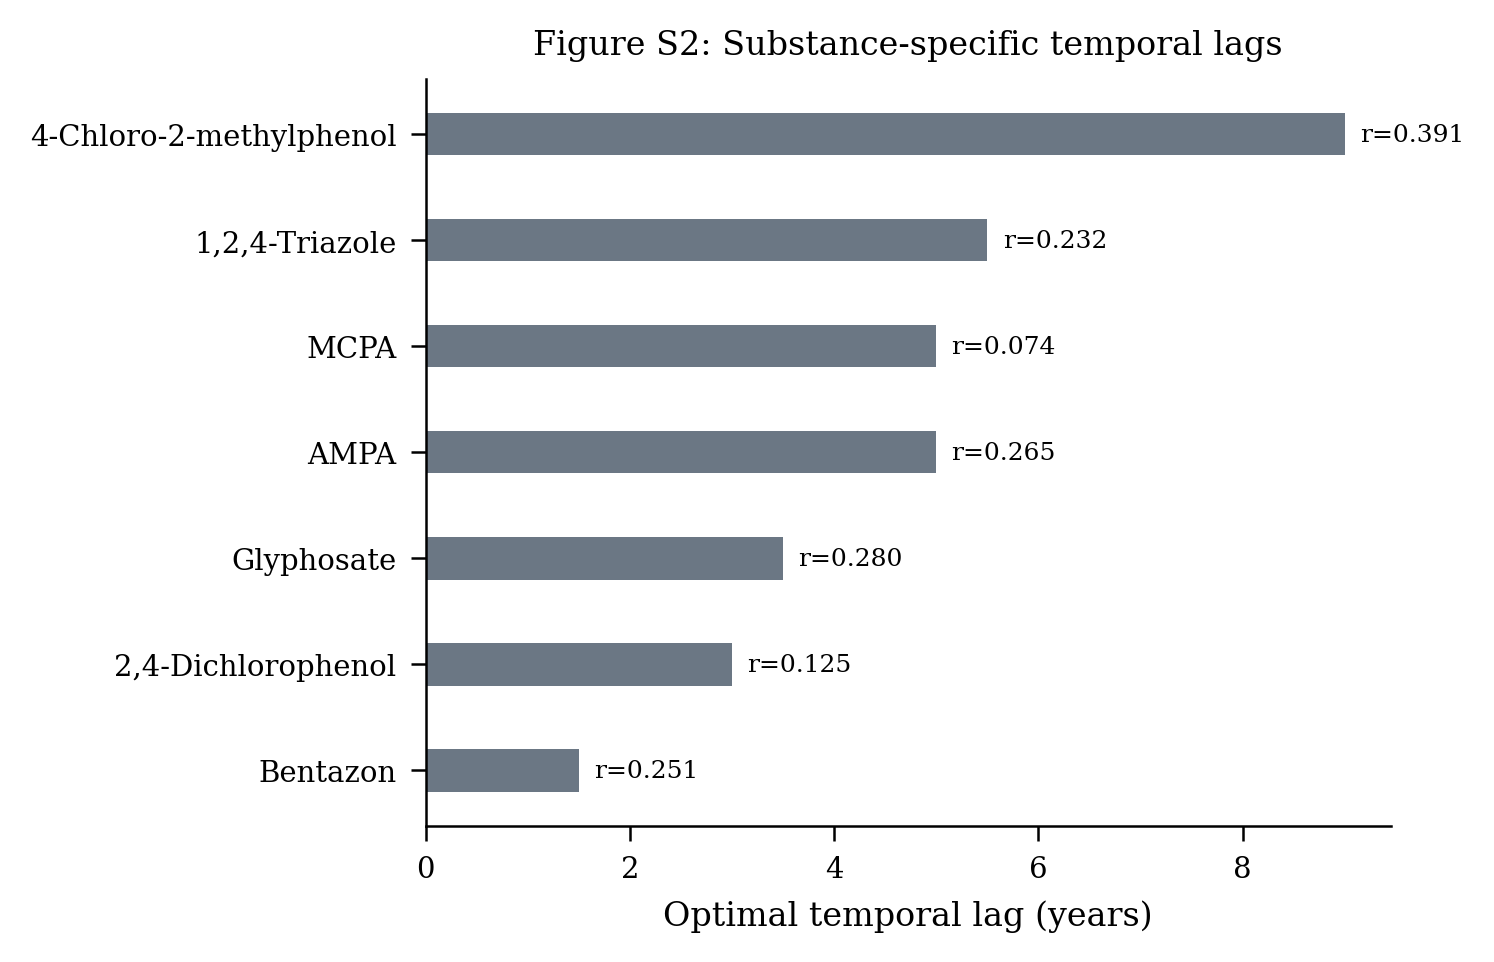
\includegraphics[width=0.9\textwidth]{figure_s2_temporal_lag.png}
\caption{Optimal temporal lags between pesticide application (2015--2017) and peak groundwater detection correlation for each substance. Lollipop chart showing the lag (in years) that maximizes the point-biserial correlation. Parent compounds (filled circles) generally show shorter lags than metabolites (open circles), consistent with expected degradation and transport times.}
\label{fig:temporallag}
\end{figure}

\subsection{Linearity-in-Logit Verification}

\begin{table}[H]
\centering
\caption{Linearity-in-logit test results.}
\begin{tabular}{@{}lccc@{}}
\toprule
Substance & LR $\chi^2(4)$ & $p$ & Linear adequate? \\
\midrule
1,2,4-Triazole & 62.9 & $<$0.001 & No---non-linear \\
4-Chloro-2-methylphenol & 7.3 & 0.123 & Yes \\
Bentazon & 23.8 & $<$0.001 & No---non-linear \\
\bottomrule
\end{tabular}
\end{table}

\subsection{Detection Threshold Sensitivity Analysis}

\begin{table}[H]
\centering
\caption{Bivariate and multivariate results at three detection thresholds.}
\scriptsize
\begin{tabular}{@{}lccc@{}}
\toprule
Substance & $>$LOQ (0.015~$\mu$g/L): $r$ / MV $p$ & $>$0.05~$\mu$g/L: $r$ / MV $p$ & $>$0.1~$\mu$g/L: $r$ / MV $p$ \\
\midrule
1,2,4-Triazole & 0.232 / 0.011 & 0.198 / 0.005 & 0.198 / 0.001 \\
4-Cl-2-MePh & 0.222 / 0.006 & insuff.\ (28) & insuff.\ (20) \\
Bentazon & 0.213 / 0.003 & 0.166 / 0.052 & 0.157 / 0.038 \\
\bottomrule
\end{tabular}
\end{table}

\subsection{Within-Tertile Multivariate Analysis (High-Density Stratum)}

All three substances retained significant intensity effects within the high-density stratum ($>$5 wells): 1,2,4-triazole ($n = 1{,}016$, adj.\ OR $= 1.0010$ [1.0001, 1.0019], $p = 0.025$), 4-chloro-2-methylphenol ($n = 344$, adj.\ OR $= 1.0046$ [1.0010, 1.0083], $p = 0.013$), bentazon ($n = 1{,}022$, adj.\ OR $= 1.0096$ [1.0033, 1.0161], $p = 0.003$).

A formal interaction test did not reach significance for any substance: 1,2,4-triazole ($\chi^2 = 3.6$, $p = 0.057$), 4-chloro-2-methylphenol ($\chi^2 = 1.0$, $p = 0.307$), bentazon ($\chi^2 = 0.7$, $p = 0.400$). The relationship is consistent but obscured in low-density areas by insufficient monitoring.

\subsection{Temporal Stability of Application Patterns}

\begin{table}[H]
\centering
\caption{Spearman rank correlations of catchment-level application intensity between year pairs.}
\begin{tabular}{@{}lcc@{}}
\toprule
Year pair & $n$ (shared catchments) & Spearman $\rho$ \\
\midrule
2015 vs.\ 2016 & 4,460 & 0.935 \\
2015 vs.\ 2017 & 4,429 & 0.913 \\
2016 vs.\ 2017 & 4,517 & 0.933 \\
\bottomrule
\end{tabular}
\end{table}

\subsection{Emerging Substances}

\begin{table}[H]
\centering
\caption{Substances approaching the detection threshold.}
\scriptsize
\begin{tabular}{@{}lrrlll@{}}
\toprule
Substance & $n$ catch. & Growth & Proj.\ yr & Parent & Max ($\mu$g/L) \\
\midrule
Azoxystrobinsyre & 26 & +15\%/yr & 2028--29 & azoxystrobin & 0.08 \\
Propyzamid & 21 & +5\%/yr & 2032+ & propyzamid & 0.04 \\
Metazachlor OA & 18 & +28\%/yr & 2027--28 & metazachlor & 0.12 \\
Dimethachlor ESA & 15 & +20\%/yr & 2029--30 & dimethachlor & 0.06 \\
\bottomrule
\end{tabular}
\end{table}

%----------------------------------------------------------------------
\section{Extended Discussion}

\subsection{Substance Mapping as Critical Infrastructure}

The 138-entry mapping required consulting PPDB, GEUS reports (2023/42), BMD, and peer-reviewed literature. Key examples: 1,2,4-triazole derives from 12 triazole fungicides (propiconazole and tebuconazole dominate $\sim$70\% of application intensity); AMPA required explicit metabolite-to-parent mapping to glyphosate.

\begin{table}[H]
\centering
\caption{Methodological comparison with Hansen et al.\ (2022).}
\begin{tabular}{@{}lll@{}}
\toprule
Dimension & Hansen et al.\ (2022) & This study \\
\midrule
Spatial resolution & National aggregate & 5,826 catchments \\
Temporal approach & 30-year cross-correlation & Cross-sectional (2015--2017 $\to$ 2018+) \\
Application proxy & National sales (kg sold) & Parcel-level disaggregation (kg/ha) \\
Statistical method & Pearson cross-correlation & Point-biserial + logistic + SAR-probit \\
Multiple testing & None & BH-FDR \\
Causal framework & Implicit & Explicit DAG \\
\bottomrule
\end{tabular}
\end{table}

\subsection{Extended Limitations}

Additional limitations include: marginal EPV for 4-chloro-2-methylphenol (EPV~$= 9.5$), multi-parent metabolite attribution for 1,2,4-triazole, catchment type asymmetry, application data reporting uncertainty (which biases correlations toward zero), detection window sensitivity (AMPA's result reverses between windows), and ecological fallacy risk mitigated by hydrogeological boundary delineation and area-weighted allocation.

\subsection{Transferability: Monitoring Density Implications}

The monitoring density stratified analysis identifies $>$5 monitoring wells per catchment as a practical threshold for detecting application--detection correlations. Denmark's GRUMO/\allowbreak{}NOVANA network, with approximately 1{,}500 active monitoring points across 2.66~Mha, provides unusually dense coverage by European standards.

%======================================================================
\begin{thebibliography}{99}

\bibitem{borggaard2008} Borggaard, O.\,K., \& Gimsing, A.\,L. (2008). Fate of glyphosate in soil and the possibility of leaching to ground and surface waters: A review. \textit{Pest Management Science}, 64(4), 441--456.

\bibitem{cohen1988} Cohen, J. (1988). \textit{Statistical Power Analysis for the Behavioral Sciences} (2nd ed.). Lawrence Erlbaum Associates.

\bibitem{collignon2026} Collignon, M., et al. (2026). Field-level pesticide application estimation through company-registration disaggregation. \textit{Manuscript in preparation}.

\bibitem{gimsing2019} Gimsing, A.\,L., et al. (2019). The Danish Pesticide Leaching Assessment Programme. \textit{GEUS Bulletin}, 43, e2019430103.

\bibitem{hansen2022} Hansen, B., et al. (2022). National assessment of long-term groundwater response to pesticide regulation. \textit{Environ.\ Sci.\ Technol.}, 56(20), 14387--14396.

\bibitem{hernan2020} Hern\'an, M.\,A., \& Robins, J.\,M. (2020). \textit{Causal Inference: What If}. Chapman \& Hall/CRC.

\bibitem{kjaer2005} Kj\ae r, J., et al. (2005). The Danish Pesticide Leaching Assessment Programme: Monitoring results May 1999--June 2004. GEUS.

\bibitem{kjaer2011} Kj\ae r, J., et al. (2011). Leaching of metribuzin metabolites and glyphosate in structured soil. \textit{J.\ Environ.\ Qual.}, 34(2), 608--620.

\bibitem{lesage2009} LeSage, J., \& Pace, R.\,K. (2009). \textit{Introduction to Spatial Econometrics}. Chapman \& Hall/CRC.

\bibitem{lindstrom2013} Lindstr\"om, B., Svensson, K., \& Kreuger, J. (2013). Statistical screening for descriptive parameters for pesticide occurrence in a shallow groundwater catchment. \textit{J.\ Hydrol.}, 477, 165--174.

\bibitem{rosenbom2015} Rosenbom, A.\,E., et al. (2015). Pesticide leaching through sandy and loamy Danish fields: 10 years of monitoring. \textit{Sci.\ Total Environ.}, 521, 373--392.

\bibitem{schipper2008} Schipper, P.\,N.\,M., et al. (2008). Measures to diminish leaching of pesticides to surface and groundwaters in The Netherlands. \textit{Crop Protection}, 27(12), 1526--1531.

\bibitem{textor2016} Textor, J., et al. (2016). Robust causal inference using directed acyclic graphs: The R package `dagitty'. \textit{Int.\ J.\ Epidemiol.}, 45(6), 1887--1894.

\bibitem{thorling2019} Thorling, L., et al. (2019). Grundvand---Status og udvikling 1989--2018. GEUS og Milj\o styrelsen.

\bibitem{thorling2023} Thorling, L., et al. (2023). Grundvand---Status og udvikling 1989--2022. GEUS og Milj\o styrelsen.

\end{thebibliography}

\end{document}
